% Page 036 — page imprimée 32
% Contenu seul : le préambule et la pagination sont gérés par meyrueis.tex


\sectiondate{La  grotte de « La Douce »}{1920}


\vspace{1.5em}

\textit{Son entrée, au dessus du Ferradou, sur le vieux chemin montant au rocher du Château, servit
longtemps de bergerie pour quelques brebis. C’est seulement en 1920 que Frank Loupiac et
son jeune cousin, Daniel Couderc\footnote{Daniel Couderc 1908-1997, fils de Léon Couderc et Madeleine de Felice, cousin germain de Frank Loupiac}, découvrirent, les premiers, le début du réseau de la
Douce\footnote{La Douce signifie « la Source ». cf André Fages : « La quête de l’eau » 2004 «
Los Adrelhans ». Le hameau « des Douze » tire aussi son nom de cette étymologie.} qu’on appelle maintenant grotte de la Porte. Philippe Chambon en est propriétaire et dispose des clefs.}

\textit{Voici le récit de cette première « exploration » tel qu’elle nous a été contée par Daniel
Couderc et enregistrée au Moulin d’Ayres au cours de l’été 1981.}

\vspace{1em}

« Comme la plupart des enfants j’ai longtemps aimé l’obscurité. Quoi de plus rassurant
lorsqu’on a deux ans de se blottir sous les couvertures tout contre la chaleur maternelle, la
conscience épanouie par de vagues et heureuses réminiscences. Plus tard vers 4 à 6
ans l’aventure se complique : elle consiste à se frayer soi-même un chemin vers la lumière,
vers le bout du lit étroitement bordé « à la française » : plus tu avances et moins il y a de
place. La tête sert de butoir, elle écarte et soulève les draps pour trouver un peu d’air, il fait
chaud, tu étouffes... Mais voilà que ton bras s’est glissé au dehors, il te tire vers la fraîcheur...
Encore un effort et tu débouches en riant tout près de tes parents dans la chambre ensoleillée
par une matinée de printemps. C’est plus tard que pour beaucoup, l’obscurité se peuple d’êtres
malfaisants : fantômes, vampires, araignées ou reptiles venus de légendes racontées par des
adultes irresponsables !!!

Il est possible que ces « histoires » aussi vieilles que l’humanité ne soient elles mêmes que le
reflet d’une crainte ancestrale venue des temps où l’obscurité était en effet pleine de pièges.
Mais c’est là une autre question...
Heureusement, et grâce à des parents éclairés, notre imagination fut préservée de ces craintes
irraisonnées, de même que celle de mon cousin Frank.

Bien qu’il soit mon aîné de 3 ans, nous nous entendions à merveille lorsque je le retrouvais à
chacun de mes séjours à Meyrueis. Il me montrait la rivière ou plutôt les trois rivières qui se
rencontrent à Meyrueis.
Pêcheur émérite il en connaissait tous les « gouffres », et lorsqu’il partait en expédition,
parfois pour toute la journée, il ne revenait jamais bredouille. Mais il aimait aussi les trous, les
grottes, les avens qui abondent dans la région et là, je le suivais avec passion.

En cette année 1920, j’avais 12 ans, lui 15 nous avions décidé de réaliser un projet qui nous
tentait depuis longtemps : nous voulions explorer la grotte de la Douce. La Douce n’est pas
une rivière, même pas un ruisseau, c’est seulement une cascade parfois impétueuse qui se
manifeste après une période de mauvais temps et de pluies abondantes. Elle jaillit du rocher et
tombe presque directement dans la Jonte juste derrière notre maison. Le trou d’où elle sort
parfaitement sec en été est trop étroit pour être remonté au-delà d’une dizaine de mètres mais
son débit lorsqu’elle fonctionne montre qu’elle est le déversoir de tout un réseau de galeries
souterraines s’étendant sous le Causse. Comment atteindre ce réseau ?»

Une ouverture triangulaire située très haut dans le rocher qui dominait notre vue du Ferradou
aurait pu être un accès. Mais après une escalade hasardeuse, accomplie au printemps avec
corde et pitons, Frank s’était rendu compte que ce trou ne permettait aucune approche
intéressante…

Restait la « Bergerie ». C’était une caverne qui s’ouvrait dans un petit champ à une centaine
de mètres au dessus de notre maison. Elle était fermée par une porte de bois à laquelle on
accédait par un chemin profond creusé entre le champ et la falaise. Le propriétaire s’appelait
« Luquet ». Il nous prêta la clef en riant : \textit{« Vous ne trouverez rien dans ma caverne, nous dit-
il, à part des crottes de brebis !… On pouvait bien y loger 200 bêtes autrefois, moi je n’ai pas
le temps de « tenir » le troupeau. »} En arrivant nous trouvâmes que la porte n’avait plus de
serrure. Des vagabonds s’étaient peut-être abrités là pendant l’hiver…

La caverne avait l’aspect d’une longue salle rectangulaire d’environ 20m sur 5, recouverte par
un rocher sans fissure. Nous marchions sur une couche élastique de très anciennes crottes de
mouton, parfaitement sèches et sans odeur. Au fond s’élevait une masse calcaire, un peu
comme un autel dans le chœur d’une église.
On pouvait en faire le tour par une galerie relativement étroite dans laquelle s’ouvraient
quelques trous à différentes hauteurs. L’un d’eux, au ras du sol, était plus profond que les
autres. C’était un véritable boyau dans lequel nous nous \textit{engageâmes d’abord en courbant le dos,
puis à genoux, enfin en rampant à mesure que la voûte s’abaissait au dessus de nous.} Le sol
était meuble, friable : un limon desséché depuis des siècles !

Frank était devant moi avec une lampe électrique. Après quelques minutes il s’arrêta un
moment, puis commença à reculer, lorsque nous nous relevâmes dans la galerie il était excité :
\textit{« j’ai peut-être trouvé ce que nous cherchions, me dit-il : Au fond du tunnel il y a un trou.
Pas bien grand mais je pouvais y passer le bras. Et de l’autre côté ma main ne rencontrait
plus de paroi, plus de sol, seulement un courant d’air. C’est sûrement une salle, peut-être
très grande, peut-être le réservoir de la Douce. Nous reviendrons demain. »}

Frank avait déjà une certaine expérience en spéléologie. Il connaissait la grotte de Dargilan, la
grande attraction touristique de la région. L’Aven Armand n’était pas encore exploité. Dans
cet immense labyrinthe il connaissait non seulement l’itinéraire ouvert au public (1h1/2 de
marche) mais encore salles et galeries restées secrètes. A l’entendre les plus belles,
naturellement ! Il savait donc ce qu’il nous fallait et lorsque nous entrâmes dans la Bergerie le
lendemain matin, nous avions un équipement rudimentaire mais suffisant : la forte lampe à
acétylène d’un vélo, une lampe électrique, 3 bougies, 2 boites d’allumettes et 3 pelotons de fil
rouge « empruntés » à la filature du Moulin d’Ayres, pour nous servir de fil d’Ariane… et une
solide pelle à charbon.

Le déblaiement du tunnel que nous pûmes approfondir d’environ 30 cm nous prit une bonne
heure, mais après ce travail nous pouvions nous y glisser à l’aise et surtout, la paroi terminale
n’était plus un obstacle : le trou était devenu une large ouverture. La lampe à acétylène nous
révéla que nous nous trouvions en haut d’une vaste salle très profonde, au sommet d’un
éboulis formé par des débris de stalagmites et stalactites éboulés sur le sol et sur lesquels, par
endroits, de nouvelles et importantes stalagmites s’étaient formées. Le même phénomène a été
observé dans l’Aven Armand et les géologues ont estimé que ces éboulis étaient dus à un
tremblement de terre ayant eu lieu il y a environ 15 000 ans.

Ce n’est pas sans émotion que nous nous sommes engagés sur la pente raide mais facile à
descendre, nous les premiers hommes… « Pense un peu, Frank, les premiers à pénétrer dans
ce mystère ! ! ! … ».

En bas se trouvait une vasque peu profonde, pleine d’une eau parfaitement limpide. Elle était
alimentée par une goutte d’eau qui tombait, à intervalles réguliers, par une sorte de cheminée
verticale qui s’ouvrait dans la voûte à moins d’un mètre du niveau de l’eau. Cette goutte
devait avoir une grande force car en tombant elle formait des éclaboussures et produisait une
note cristalline assez sonore pour être répercutée par la voûte de la grande salle. J’étais ravi ;
j’aurais voulu rester longtemps à l’écouter. Mais mon cousin voulait que nous continuions
l’exploration. Pendant plus d’une heure nous nous acharnâmes à chercher de nouvelles
galeries, mais nous n’avions pas de corde pour nous assurer et les quelques trous qu’on
pouvait discerner dans le rocher étaient trop haut pour qu’on puisse les atteindre avec nos
propres moyens.

Lorsque nous fûmes sortis Frank ne me cacha pas sa déception : \textit{« C’est vrai nous avons
trouvé une salle, me dit-il, mais elle n’a pas de stalagmites comme le clocher de Dargilan,
pas de stalactites excentriques comme à Fond de Gaume, pas de peintures rupestres comme à
Altamira, pas même un squelette d’ours ou de renard comme à Nabrigas, rien
d’intéressant… ».}
Le lendemain nous rendîmes la clé à son propriétaire lui racontant notre exploit ? \textit{« c’est ce
que je vous avais dit, concluait-il en haussant les épaules, il n’y a rien à tirer de cette
caverne, elle ne vaut même pas les frais d’une serrure ».}
Le soir un orage éclata suivi par une période de mauvais temps. C’était la fin des vacances et
des aventures.
L’année suivante, dès mon arrivée à Meyrueis, je montai à la Bergerie : la porte était toujours
sans serrure, rien ne s’opposait à une nouvelle exploration. Mon cousin n’était pas là mais
c’était sans importance. J’étais bien décidé à faire moi-même mes découvertes sans en parler à
personne, car j’avais une idée : je voulais explorer la cheminée dont nous avions vu l’entrée
au dessus de la vasque. Trois jours plus tard l’occasion se présenta : le temps était beau, ma
tante avait des visites à faire et je lui annonçais que j’allais en promenade. J’avais 3 bougies,
une lampe électrique et 2 boîtes d’allumettes. Quelques minutes après, j’étais sur les lieux
sans soupçonner que j’étais au seuil d’une expérience décisive…
Rien n’avait changé depuis l’année précédente : la terre de nos déblais se trouvait toujours à
l’entrée de notre tunnel. Lorsque je m’y glissais je retrouvais le sentiment délicieux qui me
saisissait autrefois lorsque je jouais à me perdre sous les couvertures du lit de mes parents. À
la sortie, je retrouvais le fil rouge que nous avions attaché à une stalagmite. Je descendis sans
anicroche, retrouvais la vasque et sa cheminée qui n’était pas d’un accès difficile. Je
l’escaladais sans hésiter, et à moins de 2 m. je rencontrais une galerie horizontale, assez large
qui s’ouvrait à droite et à gauche. Les parois étaient lisses le sol uni : elle avait servi de canal
il y a quelques dizaines de milliers d’années et la cheminée était le résultat d’une dislocation
sans doute provoquée par un tremblement de terre ; ses roches brutes n’avaient pas été usées
par les eaux du canal probablement tari par la même occasion. Suivant alors la galerie je
découvris d’autres fissures dans le sol. Pour épargner la lampe électrique j’avais allumé une
bougie. J’avançais pas à pas, prudemment… Soudain je me trouvais au seuil d’une
merveille !!! C’était une salle relativement petite, intime et ronde, comme un petit salon,
entièrement tapissée de cristaux brillants et translucides. J’allumai des deux autres bougies :
leur lumière était réfléchie mille, dix mille fois en faisceaux irisés d’étincelantes couleurs. Ma
présence dans cet écrin me semblait presque sacrilège, j’étais fasciné immobile tout entier
dans la joie de l’admiration.

Cinquante six ans plus tard en 1977, lors d’une courte visite à Meyrueis, j’essayai de retrouver
la bergerie. Le chemin existait toujours quoique embroussaillé mais le petit champ était
clôturé et avait une porte neuve fermée à clé. Et la tranchée qui menait à l’entrée de la grotte
avait été soigneusement remplie sur toute sa longueur par des branchages aux épines acérées.

Ma grotte était condamnée, plus dangereuse peut-être que je ne l’avais cru. Dommage...

J’aurais aimé pouvoir retrouver, ne fut-ce que pour un moment, l’obscurité totale et le
silence, un silence ponctué depuis toujours par la chute d’une goutte d’eau dans une vasque,
la même... jamais la même ! ».


\begin{center}
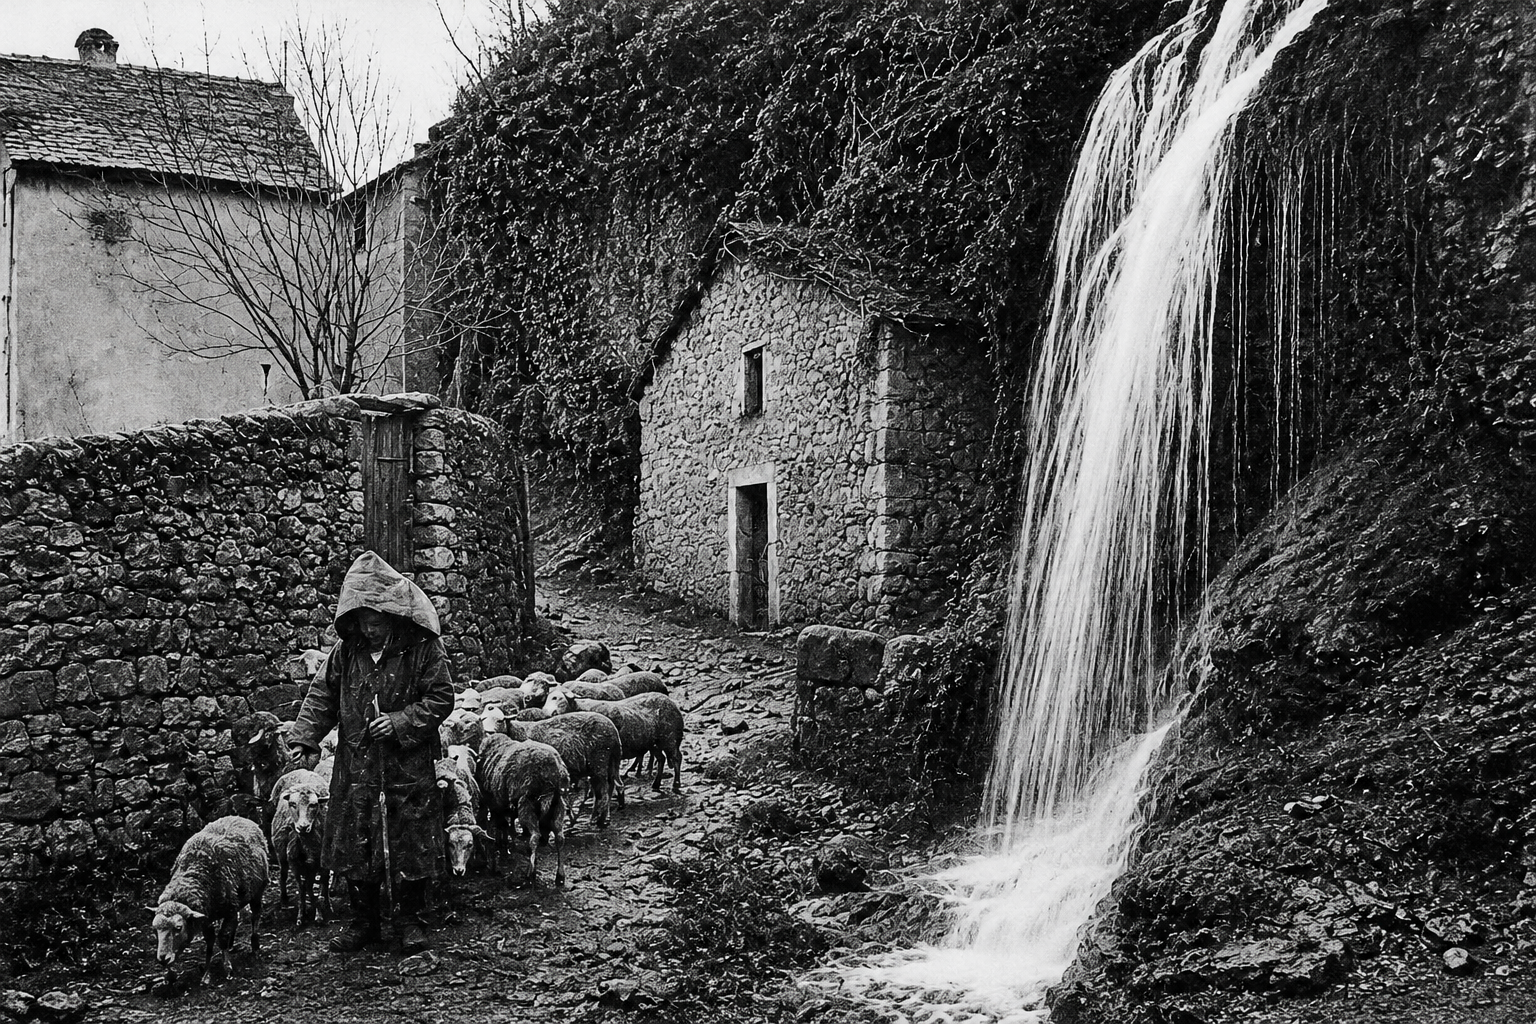
\includegraphics[width=\textwidth]{imgs/040.png}
\end{center}
